\documentclass[12pt]{article}
\usepackage{graphicx}

\usepackage{tikz}
\usetikzlibrary{positioning, calc, shapes}

\begin{document}

\section*{Labelling edges}

Use simple nodes to label those edges
\vspace{1em}

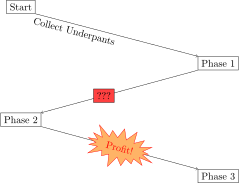
\includegraphics{_img_src/labelling-edges.pdf}

\vspace{1em}
\hrule 
\vspace{1em}

\begin{tikzpicture}
    \node[draw] (start) at (0, 8) {Start};
    \node[draw] (phase1) at (7, 6) {Phase 1};
    \node[draw] (phase2) at (0, 4) {Phase 2};
    \node[draw] (phase3) at (7, 2) {Phase 3};

    \draw[->] (start.south east) -- (phase1.north west); %% TODO, add code here;
    \draw[->] (phase1.south west) -- (phase2.north east); %% TODO, add code here;
    \draw[->] (phase2.south east) -- (phase3.north west); %% TODO, add code here;

\end{tikzpicture}

\end{document}